%----------------------------------------------------------------------------------------
%	KENAN FIRMANSYAH - MODERN TWO-COLUMN RESUME
%	Cool design with sidebar and photo
%----------------------------------------------------------------------------------------

\documentclass[11pt,a4paper]{article}

%----------------------------------------------------------------------------------------
%	PACKAGES
%----------------------------------------------------------------------------------------
\usepackage[utf8]{inputenc}
\usepackage[T1]{fontenc}
\usepackage{lmodern}
\usepackage[margin=0cm]{geometry}
\usepackage{hyperref}
\usepackage{fontawesome5}
\usepackage{xcolor}
\usepackage{tikz}
\usepackage{graphicx}
\usepackage{enumitem}
\usepackage{parskip}
\usepackage{multicol}
\usepackage{fancyhdr}
\usepackage{calc}

%----------------------------------------------------------------------------------------
%	COLORS
%----------------------------------------------------------------------------------------
\definecolor{sidebar}{RGB}{245, 245, 245}
\definecolor{mainbg}{RGB}{255, 255, 255}
\definecolor{accent}{RGB}{180, 150, 100}
\definecolor{darktext}{RGB}{40, 40, 40}
\definecolor{lighttext}{RGB}{100, 100, 100}

%----------------------------------------------------------------------------------------
%	SETTINGS
%----------------------------------------------------------------------------------------
\hypersetup{
    colorlinks=true,
    linkcolor=darktext,
    urlcolor=accent,
    pdftitle={Kenan Firmansyah - Resume},
    pdfauthor={Kenan Firmansyah}
}

\pagestyle{empty}
\setlength{\parindent}{0pt}

%----------------------------------------------------------------------------------------
%	CUSTOM COMMANDS
%----------------------------------------------------------------------------------------
\newcommand{\sidesection}[1]{%
    {\large\bfseries\MakeUppercase{#1}}\\[6pt]%
}

\newcommand{\mainsection}[1]{%
    {\large\bfseries\MakeUppercase{#1}}\\[8pt]%
}

\newcommand{\jobentry}[2]{%
    \textbf{#1}\\
    {\small\color{lighttext}#2}\\[4pt]%
}

%----------------------------------------------------------------------------------------
%	DOCUMENT - PAGE 1
%----------------------------------------------------------------------------------------
\begin{document}

% Background colors
\begin{tikzpicture}[remember picture, overlay]
    % Sidebar background
    \fill[sidebar] (current page.north west) rectangle ([xshift=6.5cm]current page.south west);
    % Main background
    \fill[mainbg] ([xshift=6.5cm]current page.north west) rectangle (current page.south east);
    % Top accent line
    \fill[accent] ([xshift=6.5cm, yshift=-1cm]current page.north west) rectangle ([yshift=-1.05cm]current page.north east);
\end{tikzpicture}

% SIDEBAR CONTENT
\begin{minipage}[t]{6cm}
\vspace{0.8cm}
\hspace{0.5cm}
\begin{minipage}[t]{5.5cm}

% PHOTO
\begin{center}
\begin{tikzpicture}
    \clip (0,0) rectangle (4.5cm, 4.5cm);
    \node[anchor=center] at (2.25cm, 2.25cm) {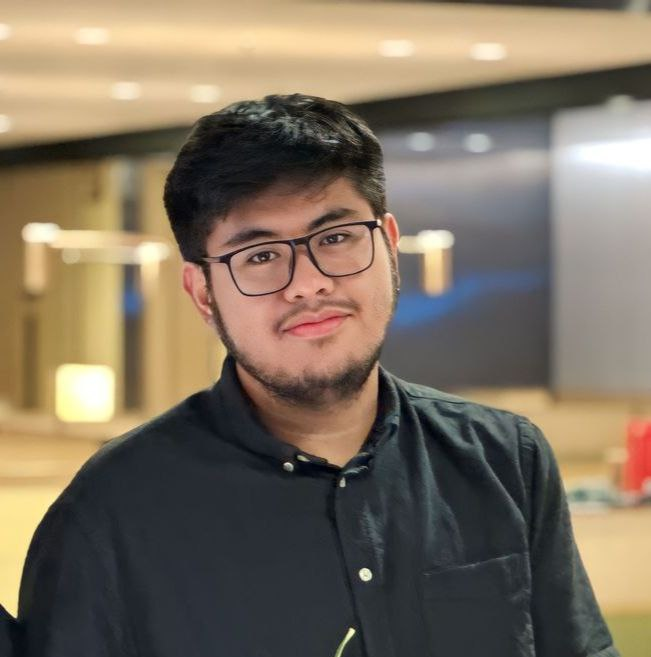
\includegraphics[width=4.5cm]{CV_ProfilePic.jpg}};
\end{tikzpicture}
\end{center}

\vspace{0.8cm}

% EDUCATION
\sidesection{Education}

\textbf{Bachelor of Computer Engineering, Major in Game Technology}\\[4pt]
{\small Electronic Engineering Polytechnic Institute of Surabaya (2020 - 2024)\\
GPA 3.67 (Cumlaude)}

\vspace{0.8cm}

% SKILLS
\sidesection{Skills}

\begin{itemize}[leftmargin=*, nosep, itemsep=4pt]
    \item Programming (Python, C++, C\#, Unreal Blueprint)
    \item Data Analysis and Visualization
    \item Mobile App Development (Figma, Swift)
    \item Game Design and Development
    \item AI and Machine Learning
\end{itemize}

\vspace{0.8cm}

% CONTACT
\sidesection{Contact}

\faIcon{linkedin} \href{https://linkedin.com/in/kenanfirmansyah}{Kenan Firmansyah}\\[6pt]
\faIcon{github} \href{https://github.com/Kenanfir}{Kenanfir}\\[6pt]
\faIcon{globe} \href{https://nandev.dev}{nandev.dev}\\[6pt]
\faIcon{phone} +6285175447540\\[6pt]
\faIcon{envelope} realkenanfir@gmail.com\\[10pt]

{\small\color{lighttext}Kalijudan, Mulyorejo, Surabaya, Jawa Timur 60114}\\[6pt]

{\small\color{lighttext}Holland Village Jakarta, Cemp. Putih, Jakarta Pusat, DKI Jakarta 10510}

\end{minipage}
\end{minipage}%
%
% MAIN CONTENT
\begin{minipage}[t]{14cm}
\vspace{0.5cm}
\hspace{0.8cm}
\begin{minipage}[t]{12.5cm}

% HEADER
{\Huge\bfseries\MakeUppercase{Kenan Firmansyah}}\\[6pt]
{\large\bfseries SOFTWARE ENGINEER | GAME DEVELOPER}\\[12pt]

{\small A dedicated and versatile tech enthusiast with a passion for innovation and a strong foundation in game programming, data science, mobile app development, and backend scripting.}

\vspace{0.6cm}

% EXPERIENCES AND PROJECTS
\mainsection{Experiences and Projects}

\jobentry{Game Developer}{Agate | 2026 Feb - 2026 May}
\begin{itemize}[leftmargin=*, nosep, itemsep=2pt, topsep=2pt]
    \item Contributed to an unannounced game project as a Game Developer.
\end{itemize}

\vspace{0.5cm}

\jobentry{Apple Developer (Learner)}{Apple Developer Academy | 2025 Feb - 2025 Dec}
\begin{itemize}[leftmargin=*, nosep, itemsep=2pt, topsep=2pt]
    \item Selected for an intensive program focused on app development, design thinking, and interdisciplinary collaboration.
    \item Gained hands-on experience in user research, UI/UX design, prototyping, and iterative testing.
    \item Worked in diverse teams to identify real-world problems and build impactful app-based solutions.
    \item \textbf{Won 1st Place at iPlay Apple Developer Academy Game Jam 2025}
\end{itemize}

\vspace{0.5cm}

\jobentry{Port \& Release Game to iOS}{Freelance (Milky Ice Jump) | 2025 Oct}
\begin{itemize}[leftmargin=*, nosep, itemsep=2pt, topsep=2pt]
    \item QA Test iOS build on Unity
    \item Implement Ad system for iOS version (\href{https://apps.apple.com/id/app/milky-ice-jump/id6751799679}{\underline{App Store Link}})
\end{itemize}

\vspace{0.5cm}

\jobentry{Game QA + Technical Support}{Ecosoft Interactive | 2025 April - 2025 June}
\begin{itemize}[leftmargin=*, nosep, itemsep=2pt, topsep=2pt]
    \item Reviewed builds and identified critical bugs, providing feedback to the team.
    \item Assisted in optimizing and preparing the game for iOS release, smoother performance, and UI adaptation.
    \item Facilitated better communication between designers and programmers to align game feel and production timelines.
\end{itemize}

\vspace{0.5cm}

\jobentry{Game Developer (Unreal Engine)}{Starpixel Studios | 2024 Oct - 2025 April}
\begin{itemize}[leftmargin=*, nosep, itemsep=2pt, topsep=2pt]
    \item Leading Developer in Multiplayer Horror Project
    \item Used Blueprint extensively, with occasional C++ integration for performance-critical systems
    \item Delivered weekly builds, managed bug tracking, and provided internal documentation
\end{itemize}

\end{minipage}
\end{minipage}

%----------------------------------------------------------------------------------------
%	PAGE 2
%----------------------------------------------------------------------------------------
\newpage

% Background for page 2
\begin{tikzpicture}[remember picture, overlay]
    % Top accent bar
    \fill[accent] (current page.north west) rectangle ([yshift=-0.8cm]current page.north east);
\end{tikzpicture}

\vspace{1.2cm}

\begin{center}
{\large\bfseries\MakeUppercase{Additional Experiences \& Projects}}
\end{center}

\vspace{0.5cm}

\hspace{1cm}
\begin{minipage}[t]{18cm}

% Section 1: Game Development
\begin{minipage}[t]{0.8cm}
{\Large\bfseries 1}
\end{minipage}%
\begin{minipage}[t]{17cm}
{\large\bfseries GAME DEVELOPMENT}\\[8pt]

\textbf{Saturated (Underwater Psychological Horror)}\\
{\small JoyBait Studio | 2025 Oct - 2025 Dec}
\begin{itemize}[leftmargin=*, nosep, itemsep=2pt, topsep=2pt]
    \item Play a role as the Project Manager and Programmer keeping track of the status of the game.
    \item Released on Mac App Store for Mac Silicon (\href{https://apps.apple.com/id/app/saturated/id6755347604}{\color{accent}\underline{App Store Link}})
\end{itemize}

\vspace{0.4cm}

\textbf{Xanthous (Thesis: AI in VR Horror Game)}\\
{\small Electronic Engineering Polytechnic Institute of Surabaya | 2023 Feb - 2024 July}
\begin{itemize}[leftmargin=*, nosep, itemsep=2pt, topsep=2pt]
    \item Developed AI systems and game mechanics using Unreal Engine.
    \item Create immersive gameplay experiences for horror game enthusiasts.
\end{itemize}

\end{minipage}

\vspace{0.8cm}

% Section 2: Publications
\begin{minipage}[t]{0.8cm}
{\Large\bfseries 2}
\end{minipage}%
\begin{minipage}[t]{17cm}
{\large\bfseries PUBLICATIONS}\\[8pt]

\textbf{Toward Adaptive VR Design: Physiological and Cognitive Predictors of Cybersickness in Serious Games}\\
{\small IJHCI, Taylor \& Francis | 2026 \textbar{} DOI: 10.1080/10447318.2026.2684064}

\vspace{0.25cm}

\textbf{Adaptive Radio System Using MetaSounds for Serious VR Game}\\
{\small IEEE Access (Vol. 13) | Nov 2, 2025 \textbar{} DOI: 10.1109/ACCESS.2025.3627544}

\vspace{0.25cm}

\textbf{Real Time Procedural Audio for Immersive Gameplay with MetaSounds}\\
{\small TCCE 2025, Trends in Computational and Cognitive Engineering | 2025}

\vspace{0.25cm}

\textbf{Dynamic Level of Difficulties Using Q-Learning and Fuzzy Logic}\\
{\small IEEE Access (Vol. 12) | Sep 12, 2024 \textbar{} DOI: 10.1109/ACCESS.2024.3457801}

\vspace{0.25cm}

\textbf{Enhancing Serious Game Experience Through In-Game Radio Using Context-Aware Recommender System}\\
{\small INASS IJIES | Sep 2, 2024 \textbar{} DOI: 10.22266/ijies2024.1031.26}

\vspace{0.25cm}

\textbf{Dynamic Day and Night Cycle Impact in a Serious VR Game}\\
{\small ICVR 2024, International Conference on Virtual Reality | 2024}

\end{minipage}

\vspace{0.8cm}

% Section 3: Other Development
\begin{minipage}[t]{0.8cm}
{\Large\bfseries 3}
\end{minipage}%
\begin{minipage}[t]{17cm}
{\large\bfseries OTHER DEVELOPMENT}\\[8pt]

\textbf{Indonesia Game Island 2026}\\
{\small JoyBait Studio Booth | Jan 23-25, 2026}
\begin{itemize}[leftmargin=*, nosep, itemsep=2pt, topsep=2pt]
    \item Logistics \& Community Manager for game expo at Ciputra World Surabaya
    \item Showcasing Tales of Tula and Saturated at the booth
\end{itemize}

\vspace{0.4cm}

\textbf{Home Server}\\
{\small Personal Project | 2023 Oct - 2023 Dec}
\begin{itemize}[leftmargin=*, nosep, itemsep=2pt, topsep=2pt]
    \item Designed and implemented a multifunctional home server serving as a Network-Attached Storage (NAS), a database server, and a computing server.
    \item Utilized Proxmox for server operating systems, showcasing proficiency in Linux-based systems.
\end{itemize}

\end{minipage}

\vspace{1cm}

\begin{center}
\href{https://nandev.dev}{\bfseries\color{accent}\underline{View More...}}\\[4pt]
{\small nandev.dev}
\end{center}

\end{minipage}

\end{document}
